% arXiv preprint. Same text as the ICGA manuscript (main.tex): abstract.tex and body.tex.
% arXiv builds it with pdflatex; upload arxiv.tex, abstract.tex and body.tex (see README.md).
\documentclass[11pt]{article}

\usepackage{iftex}
\ifXeTeX  % Tectonic runs XeTeX: use the TeX Gyre clone of Times
  \usepackage{fontspec}
  \setmainfont{texgyretermes}[Extension=.otf, UprightFont=*-regular, BoldFont=*-bold,
    ItalicFont=*-italic, BoldItalicFont=*-bolditalic]
  \setsansfont{texgyreheros}[Extension=.otf, Scale=0.95, UprightFont=*-regular,
    BoldFont=*-bold, ItalicFont=*-italic, BoldItalicFont=*-bolditalic]
\else
  \usepackage[T1]{fontenc}
  \usepackage{newtxtext,newtxmath}
\fi
\usepackage[a4paper,margin=1in]{geometry}
\usepackage{amsmath,amssymb}
\usepackage{booktabs}
\usepackage{array}
\newcolumntype{L}[1]{>{\raggedright\arraybackslash}p{#1}}  % ragged-right table text
\usepackage{pgfplots}
\pgfplotsset{compat=1.18}
\usepackage[round]{natbib}
\bibpunct{(}{)}{;}{a}{,}{,}  % (Author, year); the list in body.tex is APA 7
\usepackage{url}
\usepackage[labelsep=period,font=small,labelfont=bf]{caption}
\usepackage[colorlinks=true,linkcolor=black,citecolor=black,urlcolor=blue]{hyperref}

\newcommand{\bbh}{bb/100}
\renewcommand{\figurename}{Fig.}
\newcommand{\tablefont}{\small\centering}  % centred tables in the text font

% End matter used by body.tex. Sage defines these; a preprint keeps only the acknowledgements.
\newenvironment{acks}[1]{\section*{Acknowledgements}#1}{}
\newenvironment{dci}[1]{}{}
\newenvironment{funding}[1]{}{}

\title{Safe Opponent Adaptation in No-Limit Hold'em from Public Information}
\author{Saksham Dubey\\[4pt]
  \normalsize [School of Computer Science and Engineering], [VIT University], [Vellore], India\\
  \normalsize \texttt{saksham.dubey2024@vitstudent.ac.in}}
\date{}

\begin{document}

\maketitle

\begin{abstract}
% Abstract text, shared by main.tex (ICGA) and arxiv.tex.
The strongest poker agents approximate an equilibrium and do not adapt, so they leave value
unclaimed against imperfect players. We study how much a lightweight agent can gain by
adapting to opponents using only public information: the betting it observes and the cards
revealed at showdown. Our agent extends a Monte Carlo equity player with an opponent model
that shrinks each observed frequency toward a typical player, and with bounded adjustments
to ranges, bluffing, bet sizing and calling. With no evidence about an opponent, it plays
exactly as the base agent. In heads-up No-Limit Texas Hold'em at 100 big blinds, over
200,000 to 300,000 hands per match, the adaptive agent wins more than the base agent against
all six opponents tested: for example 65.5 against 41.4 big blinds per 100 hands (\bbh)
against an opponent who over-folds, and 234 against 105 against one that switches style to
defeat adaptation. It also beats the base agent directly by 8.4~\bbh{} (95\% interval
$\pm$3.4). All opponents are synthetic and the agent is not an equilibrium player; we state
these limits and outline the path to stronger baselines.


\medskip\noindent{\raggedright\textbf{Keywords:} Texas Hold'em, opponent modelling, safe exploitation,
Monte Carlo simulation, imperfect-information games\par}
\end{abstract}

% Body of the paper, shared by main.tex (ICGA) and arxiv.tex.

\section{Introduction}

Agents such as Libratus and Pluribus beat top professionals by playing close to an
equilibrium \citep{brown2018,brown2019}. An equilibrium strategy cannot be beaten in the long
run, but it does not try to win the most. Against a player who folds too often or bluffs too
much, it collects only what that player's mistakes happen to give away.

Human players exploit each other constantly, but exploitation carries a risk: a strategy
fitted to an opponent can itself be exploited if the reading is wrong or the opponent
changes. Methods that bound this risk exist \citep{johanson2008,ganzfried2011,ganzfried2015},
but most published agents either ignore opponents or adapt in ways that are hard to inspect.

We ask a narrower, practical question: how much can a simple, interpretable agent gain by
adapting to opponents from public information alone, and what does it give up? Our
contributions are:
\begin{enumerate}
\item An opponent model built only from what the whole table sees, including a way to label
shown-down hands as bluffs, with each statistic shrunk toward a typical player.
\item An adaptive agent that changes ranges, bluff frequency, bet size and calling thresholds
within fixed caps, and plays identically to its base agent when it has no evidence.
\item An evaluation on commodity hardware against seven opponents, including one designed to
punish adaptation, with every result reported with its 95\% interval.
\item An open implementation in Java: rules engine, agents and evaluation harness.
\end{enumerate}

\section{Related work}

\paragraph{Equilibrium agents.} Counterfactual regret minimisation (CFR) learns approximate
equilibria through self-play \citep{zinkevich2008}. DeepStack added continual re-solving
with learned value functions \citep{moravcik2017}; Libratus combined an abstract blueprint
with safe subgame solving \citep{brown2018}; Pluribus extended the approach to six players
\citep{brown2019}; ReBeL unified search and reinforcement learning \citep{brown2020}. None of
these adapts to individual opponents.

\paragraph{Opponent modelling in poker.} Early agents from the University of Alberta tracked
opponents' action frequencies to adjust their play \citep{billings1998,billings2002}.
Bayesian approaches model a distribution over opponent strategies and update it from
observed play \citep{southey2005}.

\paragraph{Safe exploitation.} Restricted Nash response computes a strategy that exploits a
model while bounding its own exploitability \citep{johanson2008}. Data-biased responses and
safe opponent exploitation bound the risk of deviating from equilibrium
\citep{ganzfried2011,ganzfried2015}.

\paragraph{Our position.} We do not compute an equilibrium. We take a simple
simulation-based agent and study bounded, interpretable adaptation on top of it, with an
evaluation designed to show both the gain and its robustness. Placing the same layer on top
of an equilibrium agent is future work (Section~\ref{sec:conclusion}).

\section{Problem setting}

We study No-Limit Texas Hold'em with blinds of 50 and 100 chips and stacks of 100 big blinds,
reset at the start of every hand. Most experiments are heads-up (two players); we also report
three- and six-player tables.

\paragraph{Information boundary.} The agent receives exactly the messages a human player's
client receives: its own hole cards, every public action with its amount, the community
cards, pot updates, and the cards of any player whose hand is turned over at showdown. It
never sees folded or unshown cards, the deck, or another seat's private messages. In the
game server this boundary is enforced in one routing class; in the evaluation harness a copy
of that router is tested to produce identical messages over 300 random hands.

\paragraph{Goal.} Given an opponent whose strategy is unknown and possibly changing,
maximise the agent's win rate while (a) playing exactly as the base agent when there is no
evidence, and (b) not losing to opponents who change style to exploit the adaptation.

\section{Method}

The agent has three parts: a base player that estimates its chance of winning by
simulation, an opponent book that records what each player does, and an adaptive layer that
turns the book into bounded changes to the base player's decisions.

\subsection{Base agent: Monte Carlo equity}

Before the flop, every one of the 1,326 starting hands is ranked by its win rate against a
random hand, estimated once from 3,000 simulated deals per strategically distinct hand with a
fixed seed. The agent opens a share of hands that widens toward the button, from 15\% in the
earliest seat to 45\% on the button, and responds to raises by pot odds.

After the flop, it estimates its equity by dealing out the unseen cards 600 times (800 for the
adaptive agent) against a range for each opponent. A range has a \emph{width}, the share of
starting hands (best first) the opponent could hold, and a \emph{connectedness}, how likely
their hand is to have hit the board, used to reject samples. Both are set from the
opponent's actions in the current hand. The agent bets for value when its equity $e$
exceeds a bar that falls with the number of opponents $n$, and calls when $e$ beats the pot
odds by a margin $m$:
\begin{gather}
e_{\text{value}} = 0.2 + \frac{0.8}{n+1}, \\
\text{call if } e \ge \frac{c}{P+c} + m, \qquad
m = \begin{cases} 0.04 & \text{on the river,}\\ 0.08 & \text{otherwise,}\end{cases}
\end{gather}
where $c$ is the amount to call and $P$ the pot. The margin grows by 0.05 when the bet has
been raised. These constants were chosen by comparing alternatives in the evaluation harness
against rule-based opponents.

\subsection{Opponent book}

For each opponent the agent counts, across all hands it observes: hands dealt; voluntary
entries into the pot; preflop raises; preflop raises faced and folded to; postflop bets faced
and folded to; postflop actions and how many were bets or raises; and, when the opponent's
cards are shown after they had bet postflop, how many such hands were weak. A shown hand
counts as weak (a bluff) if its strength against the final board is below 0.45 on a 0 to 1
scale, roughly worse than a middle pair.

Each statistic is shrunk toward a typical player's value $p_0$ with a prior weight $w$, so a
handful of hands proves little:
\begin{equation}
\hat{p} = \frac{w\,p_0 + k}{w + N},
\end{equation}
where $k$ is the number of times the event occurred in $N$ opportunities. Preflop
frequencies use $w = 12$, postflop frequencies $w = 8$ and the bluff rate $w = 4$, because
showdowns are rarer. The typical player enters 30\% of pots, raises 18\%, folds to 60\% of
preflop raises and 45\% of postflop bets, has an aggression of 0.35, and bluffs in 30\% of
shown-down betting lines.

\subsection{Adaptive decisions}

The adaptive agent overrides five of the base agent's judgements, each a function of the
opponents' estimated habits (Table~\ref{tab:adjust}).

\begin{table}[t]
\tablefont
\caption{The five adjustments and their caps.}
\label{tab:adjust}
\begin{tabular}{@{}L{0.17\textwidth}L{0.47\textwidth}L{0.28\textwidth}@{}}
\toprule
Judgement & Change & Cap \\
\midrule
Opponent's range & Width scaled by their observed raise (or entry) rate relative to
typical; connectedness scaled down for opponents caught bluffing or betting often &
Width $\times$0.4 to $\times$2.5; connectedness $\times$0.35 to $\times$1.3 \\
Bluffing & Bluff when everyone still in folds often enough for a 0.7-pot bet to profit
(Equation~\ref{eq:bluff}) & At most 65\% of eligible spots; never into three or more players \\
Value bets & Lower bar and larger bets against players who rarely fold; the reverse against
folders & Bar $\pm$0.08; size 0.4 to 1.1 of the pot \\
Calling & Smaller margin against frequent bluffers and aggressive bettors & Margin $-0.07$ to
$+0.08$ \\
Opening & Wider opening range when players behind often fold to raises & $\times$0.8 to
$\times$1.5 \\
\bottomrule
\end{tabular}
\end{table}

A bet of $b$ times the pot breaks even as a bluff when all opponents fold with probability
$b/(1+b)$, about 0.41 for $b = 0.7$. With $F$ the product of the opponents' fold-to-bet
estimates, the agent bluffs a weak hand (equity below 0.35) with probability
\begin{equation}
\label{eq:bluff}
\Pr(\text{bluff}) = \min\!\Big(0.65,\; s\cdot\big(0.15 + 2.5\,(F - \tfrac{b}{1+b} - 0.04)\big)\Big)
\end{equation}
when the edge in brackets is positive, where $s$ is 0.55 on the flop, 0.8 on the turn and 1 on
the river, since fewer bets can follow on later streets.

\subsection{Safety properties}

\paragraph{No evidence, no change.} When every estimate equals the typical player, each
override returns the base agent's value. A test confirms that the two agents make identical
decisions in 400 random spots.

\paragraph{Bounded deviation.} Every adjustment is clamped (Table~\ref{tab:adjust}), so a
mistaken or manipulated read moves the agent only so far.

\paragraph{Gradual trust.} The shrinkage prior means early reads stay close to typical.

These are engineering safeguards, not a formal guarantee of the kind restricted Nash
response provides; Section~\ref{sec:limits} discusses the difference.

\section{Experimental setup}

\paragraph{Harness.} Agents play each other on the same rules engine the game server uses,
with no network or waiting. Every hand starts at 100 big blinds; seating is shuffled each hand
and the button rotates, so no agent keeps a positional advantage. Hands are shared across
worker threads, each running its own table with its own copy of every agent's opponent book,
which persists for that table's whole share of the match. A fixed seed makes every match
exactly repeatable.

\paragraph{Metric.} Big blinds won per 100 hands (\bbh). The 95\% interval is $\pm$1.96
standard errors of the per-hand result. Results whose intervals overlap are treated as not
different.

\paragraph{Opponents.} Table~\ref{tab:opponents} lists the opponents. Four are extreme by
design, so that the gain from each kind of adjustment can be seen.

\begin{table}[t]
\tablefont
\caption{Opponents used in the evaluation.}
\label{tab:opponents}
\begin{tabular}{@{}L{0.17\textwidth}L{0.5\textwidth}L{0.25\textwidth}@{}}
\toprule
Opponent & Behaviour & Role \\
\midrule
Easy & Rule-based starting hands and hand strength; loose & Weak but reasonable \\
Solid & Same rules without the loose habits & Sound, non-adaptive \\
Simulation & The base agent of Section 4.1 & Our own baseline \\
Caller & Never folds, never raises & Extreme: over-calls \\
Maniac & Bets or raises 65\% of the time regardless of cards & Extreme: over-aggressive \\
Over-folder & Sound before the flop; afterwards folds to any bet without a strong hand &
Extreme: over-folds \\
Chameleon & Alternates between over-folder and caller every 1,500 decisions & Designed to
punish adaptation \\
\bottomrule
\end{tabular}
\end{table}

\paragraph{Hardware.} A 12-core consumer laptop. The harness plays about 100,000 hands per
second with rule-based agents; simulation agents are slower because of the equity sampling.

\section{Results}

The adaptive agent won more than the base agent against every opponent, with no overlap
between intervals in any match (Fig.~\ref{fig:headsup}, Table~\ref{tab:headsup}).

\subsection{Heads-up against each opponent}

\begin{table}[t]
\tablefont
\caption{Heads-up win rates of the base (simulation) and adaptive agents, in \bbh{} with 95\%
intervals. Seed 5, 100 big blinds.}
\label{tab:headsup}
\begin{tabular}{@{}lrrr@{}}
\toprule
Opponent & Hands & Base agent & Adaptive agent \\
\midrule
Caller      & 200,000 & 345.0 $\pm$ 5.4  & 1079.4 $\pm$ 15.4 \\
Maniac      & 200,000 & 292.8 $\pm$ 11.0 & 562.8 $\pm$ 15.2 \\
Chameleon   & 200,000 & 105.2 $\pm$ 2.8  & 233.8 $\pm$ 6.4 \\
Over-folder & 200,000 & 41.4 $\pm$ 1.3   & 65.5 $\pm$ 1.3 \\
Solid       & 300,000 & 35.5 $\pm$ 1.7   & 57.1 $\pm$ 1.6 \\
Easy        & 300,000 & 28.9 $\pm$ 2.3   & 42.1 $\pm$ 2.5 \\
\bottomrule
\end{tabular}
\end{table}

\begin{figure}[t]
\centering
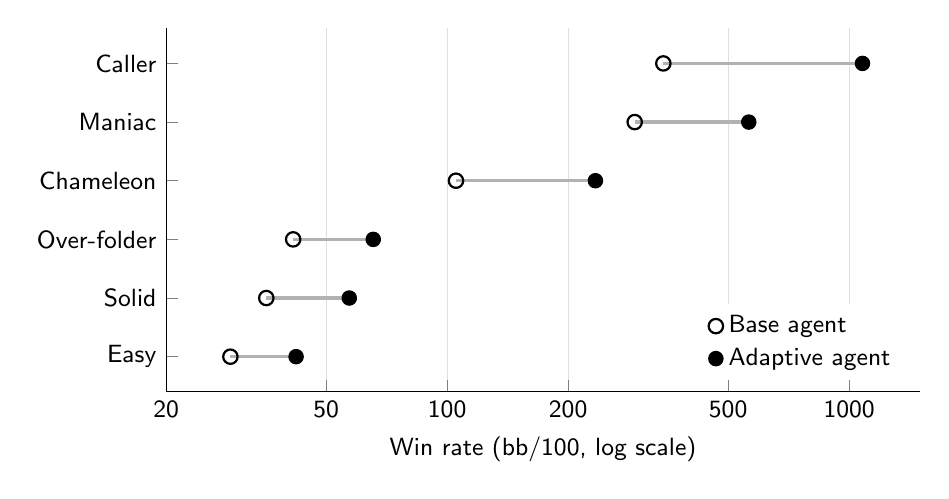
\begin{tikzpicture}
\begin{semilogxaxis}[
  width=0.92\textwidth, height=6.2cm,
  xmin=20, xmax=1500,
  ymin=0.4, ymax=6.6,
  ytick={1,2,3,4,5,6},
  yticklabels={Easy,Solid,Over-folder,Chameleon,Maniac,Caller},
  xlabel={Win rate (\bbh, log scale)},
  xtick={20,50,100,200,500,1000},
  xticklabels={20,50,100,200,500,1000},
  tick label style={font=\small\sffamily},
  label style={font=\small\sffamily},
  axis lines*=left, ymajorgrids=false, xmajorgrids=true,
  grid style={gray!25},
  legend style={at={(0.98,0.03)},anchor=south east,draw=none,font=\small\sffamily},
  legend cell align=left,
]
\foreach \y/\a/\b in {1/28.9/42.1, 2/35.5/57.1, 3/41.4/65.5, 4/105.2/233.8, 5/292.8/562.8, 6/345.0/1079.4} {
  \edef\tmp{\noexpand\draw[gray!60, line width=1.2pt] (axis cs:\a,\y) -- (axis cs:\b,\y);}
  \tmp
}
\addplot[only marks, mark=o, mark size=2.6pt, black, thick]
  coordinates {(28.9,1) (35.5,2) (41.4,3) (105.2,4) (292.8,5) (345.0,6)};
\addlegendentry{Base agent}
\addplot[only marks, mark=*, mark size=2.6pt, black]
  coordinates {(42.1,1) (57.1,2) (65.5,3) (233.8,4) (562.8,5) (1079.4,6)};
\addlegendentry{Adaptive agent}
\end{semilogxaxis}
\end{tikzpicture}
\caption{Heads-up win rate of the base agent (open circles) and the adaptive agent (filled
circles) against each opponent, on a log scale. The line joins the two agents' results
against the same opponent. 95\% intervals are smaller than the markers (Table~\ref{tab:headsup}).}
\label{fig:headsup}
\end{figure}

The gain is largest against the most one-sided opponents (the caller and the maniac) and
smallest against the sound rule-based players, as expected. Against the chameleon, built to
punish adaptation, the agent still more than doubled the base agent's win rate.

\subsection{Direct comparison and larger tables}

\begin{table}[t]
\tablefont
\caption{Direct comparison and multi-player tables, in \bbh{} with 95\% intervals.}
\label{tab:tables}
\begin{tabular}{@{}L{0.36\textwidth}rL{0.4\textwidth}@{}}
\toprule
Match & Hands & Result \\
\midrule
Adaptive against base, heads-up & 200,000 & Adaptive $+8.4 \pm 3.4$ \\
Three-handed: the agent and two over-folders & 200,000 & Adaptive $+42.8 \pm 1.9$; base
$+23.3 \pm 2.0$ \\
Six-handed, sound agents only (two adaptive, two base, two Solid) & 600,000 & Adaptive $+7.8$
and $+3.9$ ($\pm 2.7$); base $-2.1$ and $-3.8$ ($\pm 2.9$); Solid $-1.5$ and $-4.3$ ($\pm 2.2$) \\
Six-handed with weak players (adaptive, base, Solid, two Easy, Caller) & 600,000 & Adaptive
$+628 \pm 9$; base $+371 \pm 6.5$ \\
\bottomrule
\end{tabular}
\end{table}

Table~\ref{tab:tables} shows that at a table of sound agents the advantage is small and only
one of the two adaptive seats clears its interval: there is little to exploit. In a live
server session of 300 hands against a stand-in that only checks and calls, two adaptive
agents won 165,233 and 148,557 chips against the base agent's 25,296. This is anecdotal and
not used as evidence.

\section{Limitations and threats to validity}
\label{sec:limits}

\paragraph{Synthetic opponents.} Every opponent was written by us, and four of them are
extreme by design. Real players are less one-sided, so gains against people will be smaller.
The chameleon tests robustness to one switching pattern, not to an adversary who models our
agent.

\paragraph{No equilibrium baseline.} The base agent is a heuristic simulation player, not an
approximate equilibrium, so we cannot yet state how exploitable either agent is. The ``no
loss'' result is against our own non-adaptive agents only.

\paragraph{No external benchmark or human study.} We have not played public benchmark agents
such as Slumbot, and the only games against people so far are informal.

\paragraph{Tuning on the same opponents.} The base agent's constants were tuned against the
rule-based opponents it is later measured against. The adaptive layer was not tuned at all.

\paragraph{Variance reduction.} Results use plain matches, not duplicate deals or AIVAT, so
intervals are wider than they need to be.

\paragraph{Ablations.} We have not yet measured the contribution of each adjustment on its
own, or how quickly the gain appears as hands are observed.

\paragraph{Informal safety.} The caps bound how far the agent deviates but do not bound its
exploitability in the formal sense of restricted Nash response.

\section{Conclusion and future work}
\label{sec:conclusion}

A simple opponent model built from public information, combined with bounded adjustments,
roughly doubles a simulation agent's win rate against several kinds of flawed opponent,
survives an opponent that switches style to defeat it, and still beats the unadapted agent
directly. It needs no training, runs on a laptop, and every decision can be traced to a named
statistic.

The next steps, in order, are: ablations (each adjustment switched off in turn) and learning
curves (gain against hands observed); a human study with several players and a few hundred
hands each; an equilibrium baseline, a self-play Monte Carlo CFR blueprint for heads-up play
validated on Kuhn and Leduc poker and followed by real-time search, with the opponent model
placed on top of it as a restricted Nash response so that the informal caps become a formal
bound; matches against Slumbot; and reporting of compute cost (core-hours and memory) for
each stage alongside published agents.

\begin{acks}{[To be added.]}
\end{acks}

\begin{dci}{The author declares no potential conflicts of interest with respect to the research,
authorship, and/or publication of this article.}
\end{dci}

\begin{funding}{The author received no financial support for the research, authorship, and/or publication
of this article.}
\end{funding}

\section*{Data availability statement}
The source code of the game engine, agents and evaluation harness, and the commands and seeds
needed to reproduce every match in this article, will be made publicly available
at [repository link] on publication.

\section*{Responsible use}
The agent was built for research and teaching on a local network. It must not be used on
real-money poker sites.

\begin{thebibliography}{11}
\setlength{\itemsep}{0pt}

\bibitem[Billings et~al.(1998)]{billings1998}
Billings, D., Papp, D., Schaeffer, J., \& Szafron, D. (1998). Opponent modeling in poker. In
\emph{Proceedings of the Fifteenth National Conference on Artificial Intelligence (AAAI-98)}
(pp.~493--499). AAAI Press.

\bibitem[Billings et~al.(2002)]{billings2002}
Billings, D., Davidson, A., Schaeffer, J., \& Szafron, D. (2002). The challenge of poker.
\emph{Artificial Intelligence}, \emph{134}(1--2), 201--240.

\bibitem[Brown et~al.(2020)]{brown2020}
Brown, N., Bakhtin, A., Lerer, A., \& Gong, Q. (2020). Combining deep reinforcement learning
and search for imperfect-information games. In \emph{Advances in Neural Information
Processing Systems 33} (pp.~17057--17069).

\bibitem[Brown \& Sandholm(2018)]{brown2018}
Brown, N., \& Sandholm, T. (2018). Superhuman AI for heads-up no-limit poker: Libratus beats
top professionals. \emph{Science}, \emph{359}(6374), 418--424.

\bibitem[Brown \& Sandholm(2019)]{brown2019}
Brown, N., \& Sandholm, T. (2019). Superhuman AI for multiplayer poker. \emph{Science},
\emph{365}(6456), 885--890.

\bibitem[Ganzfried \& Sandholm(2011)]{ganzfried2011}
Ganzfried, S., \& Sandholm, T. (2011). Game theory-based opponent modeling in large
imperfect-information games. In \emph{Proceedings of the 10th International Conference on
Autonomous Agents and Multiagent Systems} (pp.~533--540).

\bibitem[Ganzfried \& Sandholm(2015)]{ganzfried2015}
Ganzfried, S., \& Sandholm, T. (2015). Safe opponent exploitation. \emph{ACM Transactions on
Economics and Computation}, \emph{3}(2), Article~8.

\bibitem[Johanson et~al.(2008)]{johanson2008}
Johanson, M., Zinkevich, M., \& Bowling, M. (2008). Computing robust counter-strategies. In
\emph{Advances in Neural Information Processing Systems 20} (pp.~721--728).

\bibitem[Morav\v{c}\'{i}k et~al.(2017)]{moravcik2017}
Morav\v{c}\'{i}k, M., Schmid, M., Burch, N., Lis\'{y}, V., Morrill, D., Bard, N., Davis, T.,
Waugh, K., Johanson, M., \& Bowling, M. (2017). DeepStack: Expert-level artificial
intelligence in heads-up no-limit poker. \emph{Science}, \emph{356}(6337), 508--513.

\bibitem[Southey et~al.(2005)]{southey2005}
Southey, F., Bowling, M., Larson, B., Piccione, C., Burch, N., Billings, D., \& Rayner, C.
(2005). Bayes' bluff: Opponent modelling in poker. In \emph{Proceedings of the 21st
Conference on Uncertainty in Artificial Intelligence} (pp.~550--558).

\bibitem[Zinkevich et~al.(2008)]{zinkevich2008}
Zinkevich, M., Johanson, M., Bowling, M., \& Piccione, C. (2008). Regret minimization in
games with incomplete information. In \emph{Advances in Neural Information Processing
Systems 20} (pp.~1729--1736).

\end{thebibliography}


\end{document}
